\noindent \rule{\textwidth}{0.2pt}

\noindent Datum der Vorlesung : 27.10.2014

\noindent Autor : Hinnerk van Bruinehsen

\noindent email :  h.v.bruinehsen@fu-berlin.de

\noindent \rule{\textwidth}{0.2pt}


\section*{Höhere Algorithmik - 4. Vorlesung}
\subsection*{Bestimmung des Maximums und des Minimums von $n$ Zahlen}
\textbf{Problemstellung:}
Gegeben sind die Zahlen $a_1,...,a_n$. Gesucht werden das Maximum sowie das Minimum von diesen zahlen.\\
Will man entweder nur das Maximum oder nur das Minimum dieser Zahlen bestimmen, vergleicht man die erste Zahl mit der zweiten. Je nach gesuchtem Ergebnis muss man entweder den größeren oder den kleineren der beiden Werte mit dem nächsten Wert vergleichen. Das ganze wird fortgesetzt, bis alle Zahlen miteinander verglichen wurden.\\
Aus diesem Algorithmus folgt, dass zur Bestimmung des Maximums allein $n-1$ Vergleiche ausreichen. Genauso reichen zur Bestimmung des Minimums $n-1$ Vergleiche.\\
In der Summe sind dies $2n-2$ Vergleiche. Die asymptotische Laufzeit liegt in $\mathcal{O}(n)$.\\
Anschaulich ist auch sofort klar, dass es unmöglich ist, eine bessere als lineare Laufzeit zu erreichen, da sämtliche Zahlen betrachtet werden müssen. Daher ist dies einer der wenigen Fälle in dieser Vorlesung, in der die Konstante betrachtet und verbessert werden soll.\\
\textbf{Optimierung:} Für $n \geq 2$ kann das Maximum kann nicht gleichzeitig das Minimum sein (und umgekehrt). Hieraus kann gefolgert werden, dass nur $2n-3$ Vergleiche benötigt werden.\\

\subsubsection*{Teile und herrsche}
Wir betrachten die Teilfolgen $L$ (links) und $R$ (rechts) mit $\lfloor \frac{n}{2}\rfloor$ und $\lceil \frac{n}{2}\rceil$ Elementen.\\
Das maximale Elemement der linken Teilfolge $L$ sei $l_{max}$, das minimale $l_{min}$. Analog dazu seien $r_{max}$ das maximale und $r_{min}$ das minimale Element der rechten Teilfolge $R$.\\

Bestimme $l_{min},l_{max}, r_{min}, r_{max}$\\
\begin{align*}
    T(n)&= \text{ Anzahl der Vergleiche}\\
    \\
    T(n)&=T(\lfloor \frac{n}{2}\rfloor) + T( \lceil \frac{n}{2}\rceil) +2 \\
    T(1)&=0\\
    T(2)&=1\\
    T(3)&=3=2+1+0\\
    T(4)&=4=2+1+1 \underline{< 2n-3}\\
\end{align*}
Zur Bestimmung des gesammten Maximums benötigen wir zwei weitere Vergleiche: Das maximale Element von der Gesammtfolge ist das Maximum von $l_{max}$ und $r_{max}$, das minimale Element der Gesamtfolge ist das Minimum von $l_{min}$ und $r_{min}$.\\

Analyse falls $n$ eine Zweierpotenz ist ($n=2^k$):\\
\begin{align*}
    T(n)&= 2T(\frac{n}{2})+2\\
\end{align*}

\underline{Ansatz:} $T(n) = A n +B$ (lineare Funktion)\\
Durch Einsetzen unseres Ansatzes erhalten in die Rekursionsgleichung folgt:\\
\begin{align*}
    An+B&=2(A\frac{n}{2}+B)+2\\
        &=An+2B+2 &&|(-An-B)\\
    0&=B+2 &&|(-2)\\
    B&=-2\\
\end{align*}
Bestimmung von $A$ durch Einsetzen von $B=-2$ in den Ansatz:\\
\begin{align*}
    T(n)&=An+B &\text{ für den Fall }T(2)=1\text{ folgt:}\\
    T(2)&=A2+B=1 \\
    T(2)&=A2-2=1 &(+2)\\
    2A&=3 & (/2)\\
    A&=\frac{3}{2}\\
\end{align*}

Für $A=\frac{3}{2}$ und $B=-2$ erfüllt $A\cdot n +B$ also die Rekursion.
Wir erhalten also als Lösung für den Fall $n=2^k$ ($n$ ist Zweierpotenz):
\begin{align*}
T(n)&=\frac{3}{2}n-2\\
\end{align*}

\subsubsection*{Verschiebung im Wertebereich}
Eine leicht zu lösende Rekursion hat zum Beispiel die Form: $h(n) = 2h (\frac{n}{2}) = 4 h(\frac{n}{4}) \Rightarrow h(n)=\underline{an}$\\
Schwieriger ist es, wenn die Gleichung einen Störfaktor enthält:  $f(n)=2f(\frac {n}{2})+\underbrace{2}_{\text{Störfaktor}}$\\
\begin{align*}
    f(n)&=2f(\frac{n}{2})+2 &|(+2)\\
    \Leftrightarrow f(n)+2&= 2f(\frac{n}{2})+4 & (2\text{ ausklammern})\\
    \Leftrightarrow f(n)+2& = 2 (f(\frac{n}{2})+2)\\
    \text{ definiere } g(n)&=f(n)+\underbrace{2}_{\text{Durch Ansatz}}\\
    g(n)&=2 g(\frac{n}{2})&\text{ additiver Störfaktor ist weg.}\\
    g(n)&=f(n)+c\\
    f(n)&=2 f(\frac{n}{2})+2\\
    f(n)&=g(n)-c\\
    g(n)-c&= 2(g(\frac{n}{2})+2= 2 g(\frac{n}{2})-2c+2\\
    -c&=-2c+2\\
    c&=2\\
\end{align*}
%Bild 1
\begin{figure}[h]
    \begin{center}
        %TODO
        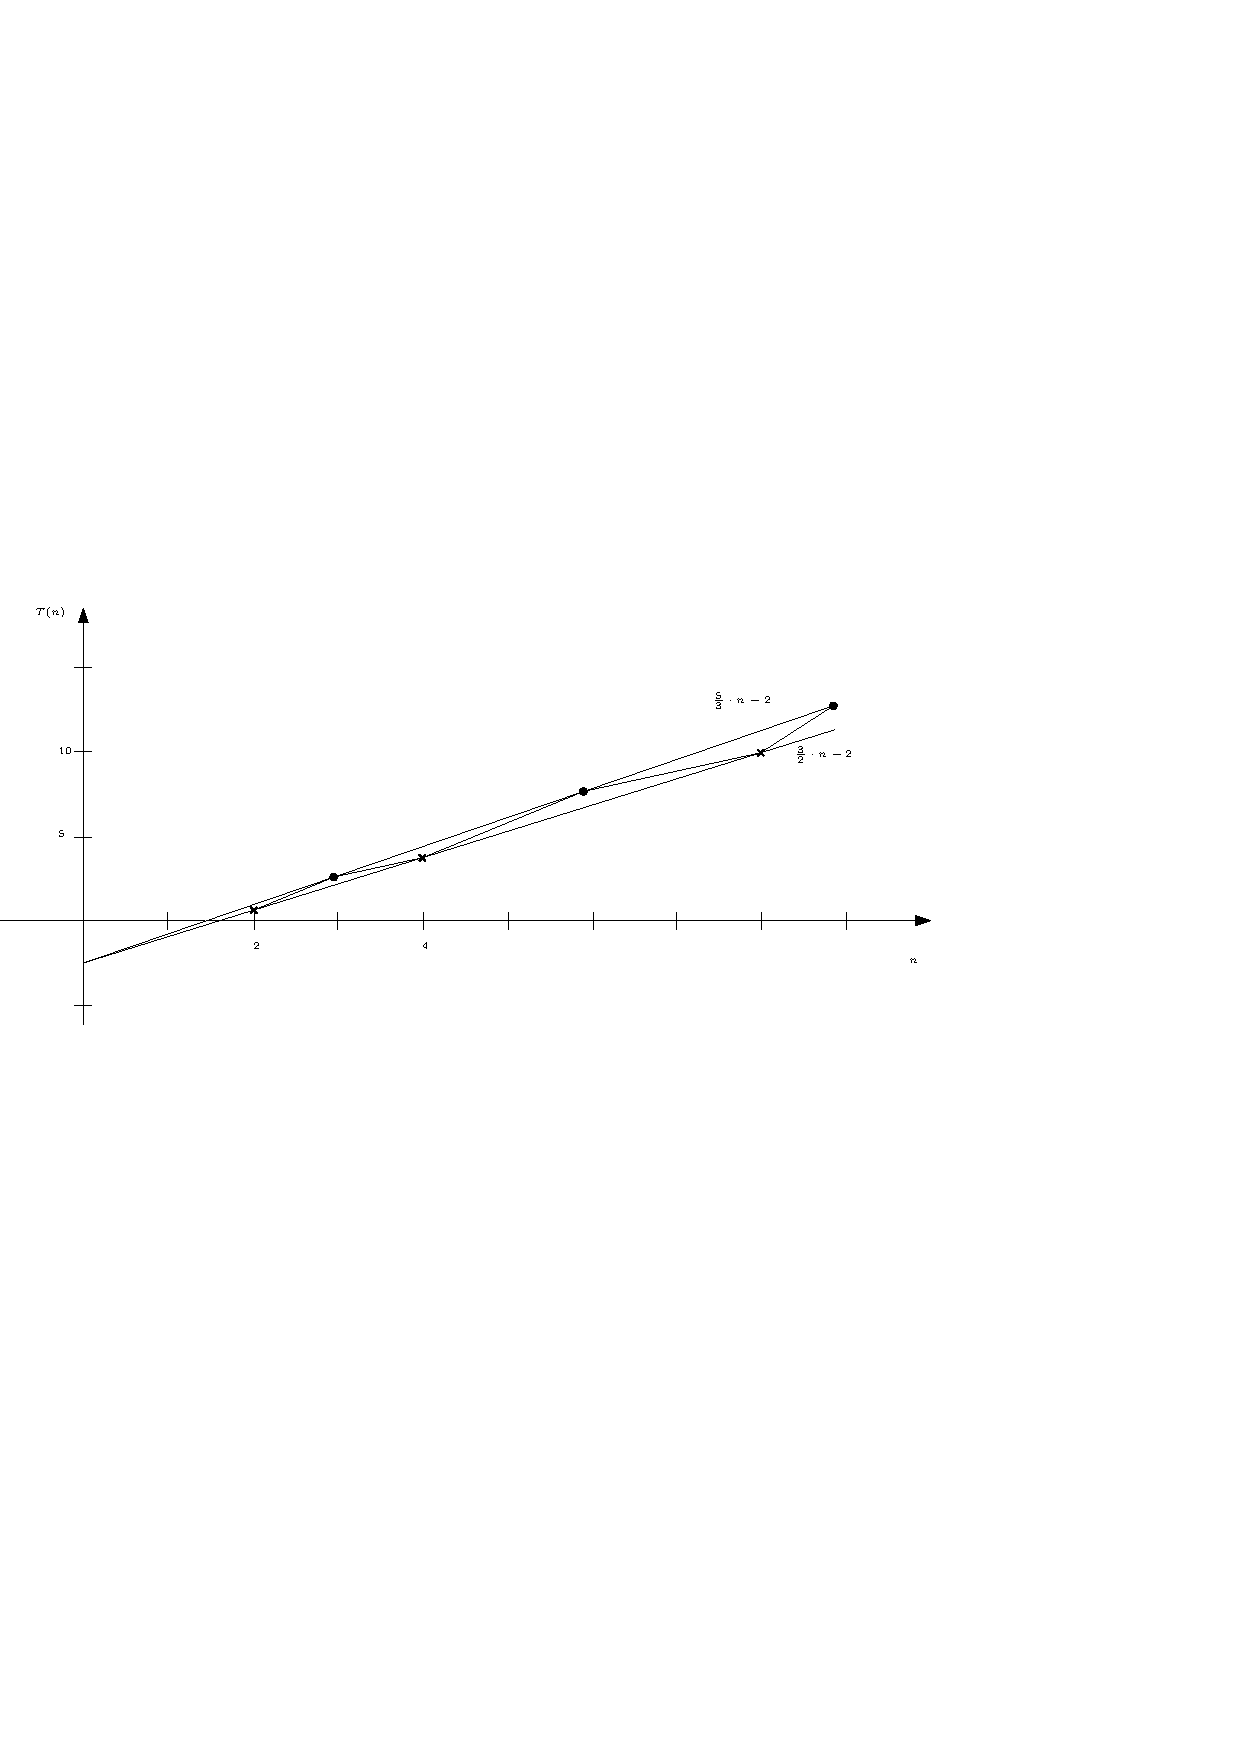
\includegraphics[width=\textwidth]{../officalscript/figures/vl4_fig_1.pdf}
        \label{fig:graph}
    \end{center}
\end{figure}
%
\textbf{Einschub:}\\
Beispiel: (Fibonacci-Folge mit Störfaktor)\\
\begin{align*}
    a_n &= a_{n-1}+a_{n-2}+3 &|(+3)\\
    (a_n+3) &=  (a_{n-1}+3) + (a_{n-2}+3)&\text{Fibonacci um 3 verschoben}\\
\end{align*}
\subsubsection*{Verschiebung im Definitionsbereich}
Ähnlich, wie die Verschiebung im Wertebereich funktioniert die Verschiebung im Definitionsbereich.\\
\textbf{Beispiel:}\\
\begin{align*}
g(n)  &=2\left(g(\lfloor \frac{n+3}{2}\rfloor)\right)&\text{substituiere } n =m+3\\
g(m+3)&=2\left(g(\lfloor \frac{m+6}{2}\rfloor)\right)\\
g(m+3)&=2\left(g(\lfloor \frac{m}{2}+\frac{6}{2}\rfloor)\right)\\
g(m+3)&=2\left(g(\lfloor \frac{m}{2}+3\rfloor)\right)\\
g(m+3)&=2\left(g(\lfloor \frac{m}{2}\rfloor+3)\right)
\end{align*}
Wir setzen $h(n)=g(n+3)$ und erhalten:\\
\begin{align*}
    h(n)&=2\left(h(\lfloor \frac{n}{2}\rfloor)\right)
\end{align*}
Auf diese Art haben wir den Störfaktor innerhalb des Funktionsaufrufs beseitigt und könnten jetzt regular mit der Bearbeitung dieser Aufgabe weitermachen.

\subsubsection*{Erweiterung auf nicht-2er Potenzen}
\begin{figure}[h]
    \begin{center}
        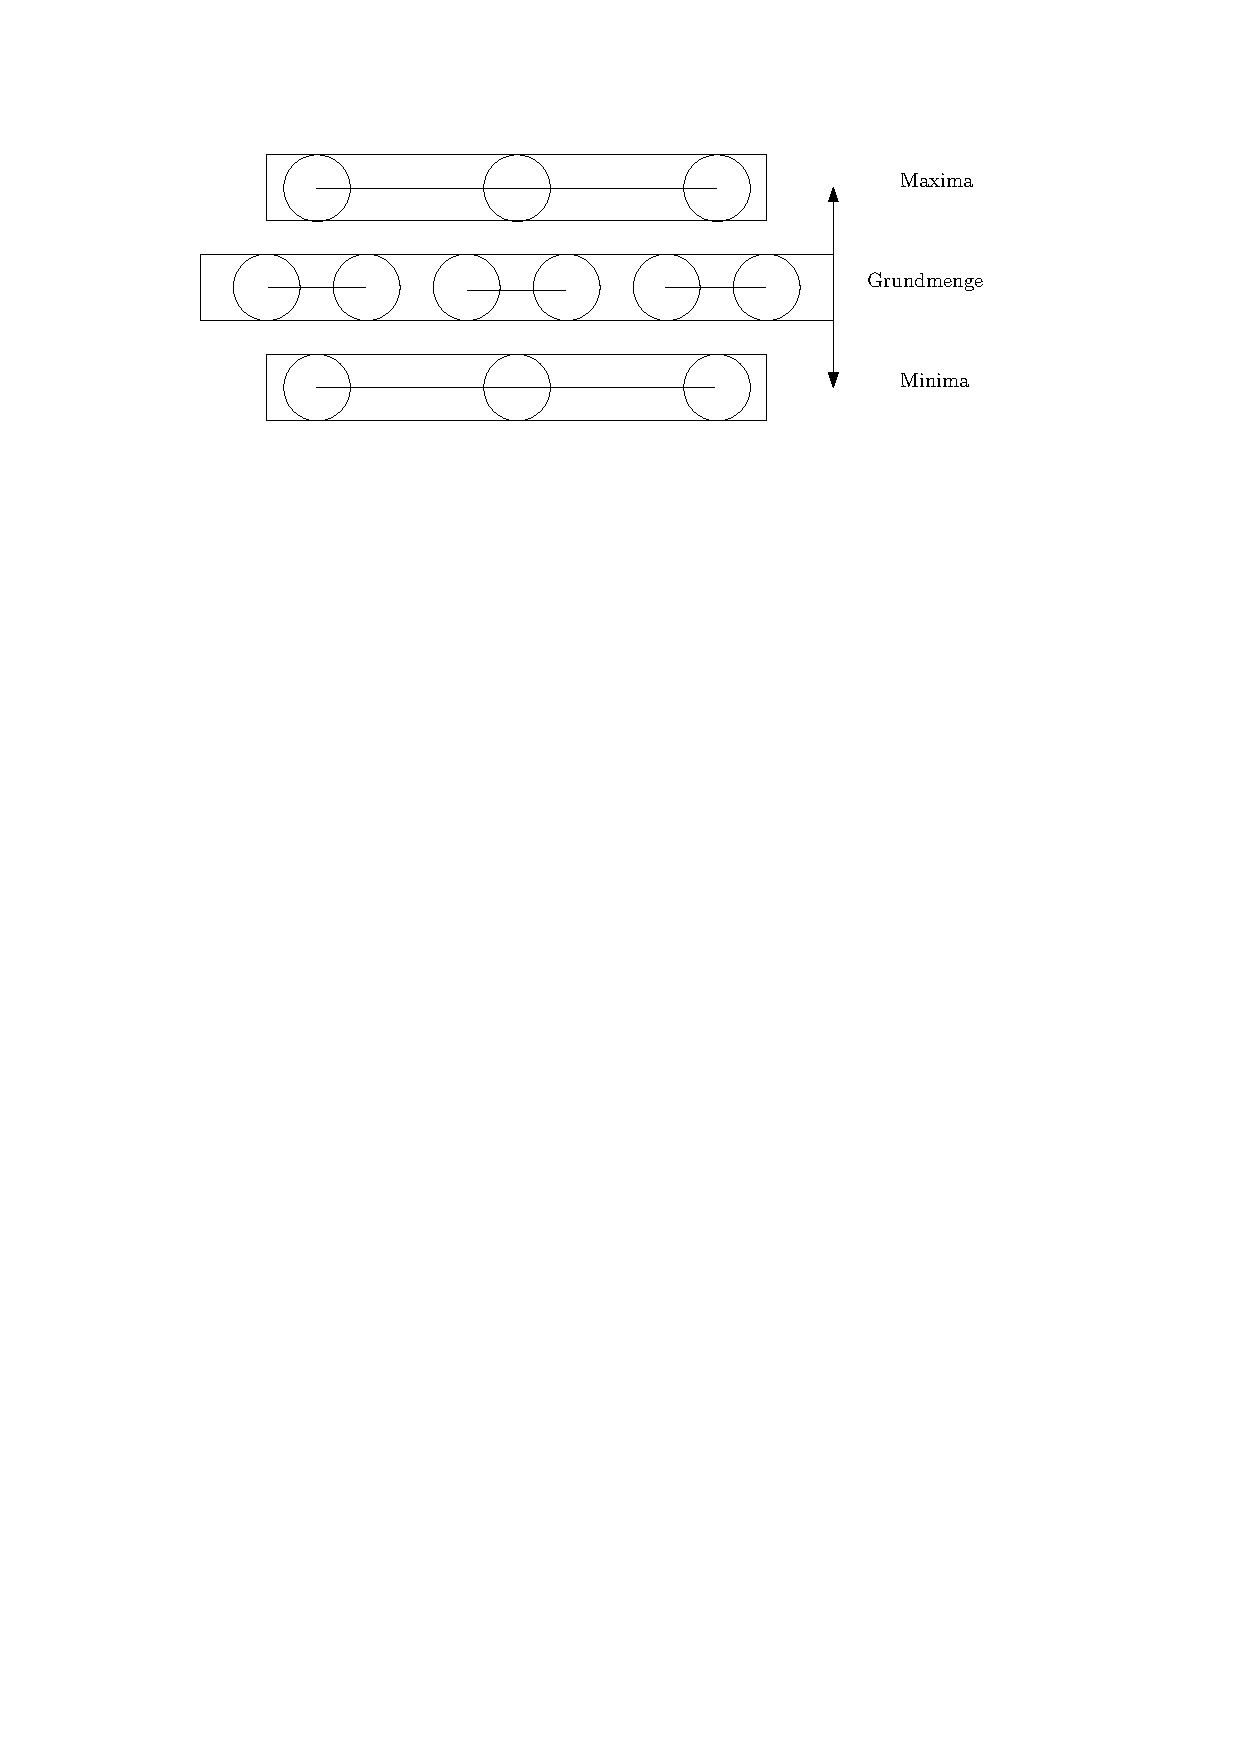
\includegraphics[width=10cm ]{../GFX/vl4_fig_comp.pdf}
        \caption{Vergleiche zum Finden von Maxima und Minima}
    \end{center}
\end{figure}
Sei $M$ eine $n$ elementige Menge. Zur Vereinfachung gehen wir davon aus, dass $n$ eine gerade Zahl ist. Wir bilden nun $\frac{n}{2}$ Paare und vergleichen diese miteinander. Hierfür benötigen wir $\frac{n}{2}$ Vergleiche.\\
Wir teilen die Elemente in zwei $\frac{n}{2}$ elementige Untermengen (ähnlich, wie bei Mergesort), von denen eine die Maxima, die andere die Minima aus den vorangegangenen Vergleichen enthält. Beide Untermengen haben nun eine ungerade Anzahl an Elementen. Wir vergleichen wieder paarweise die Maxima und die Minima. Dafür benötigen wir jeweils $\frac{n}{2}-1$ Vergleiche:\\
$\left.\begin{array}{l}
\frac{n}{2}\\
\frac{n}{2}-1\\
\frac{n}{2}-1\\
\end{array}\right\rbrace 3\frac{n}{2}-2$

Insgesamt benötigen wir also $\frac{3}{2}n-2$ Vergleiche - und damit genauso viele wie für den Fall dass $n$ als Zweierpotenz darstellbar ist. Das Verfahren funktioniert nach dem Bottom-Up Prinzip.

\subsection*{Multiplikation von zwei n-stelligen Zahlen}
Gegeben ist eine Basis $B$, z.B. $B=2$ (binär) oder $B=10$ (dezimal) oder $B=2^{32}$\\
%Bild 2
\begin{figure}[h]
    \begin{center}
        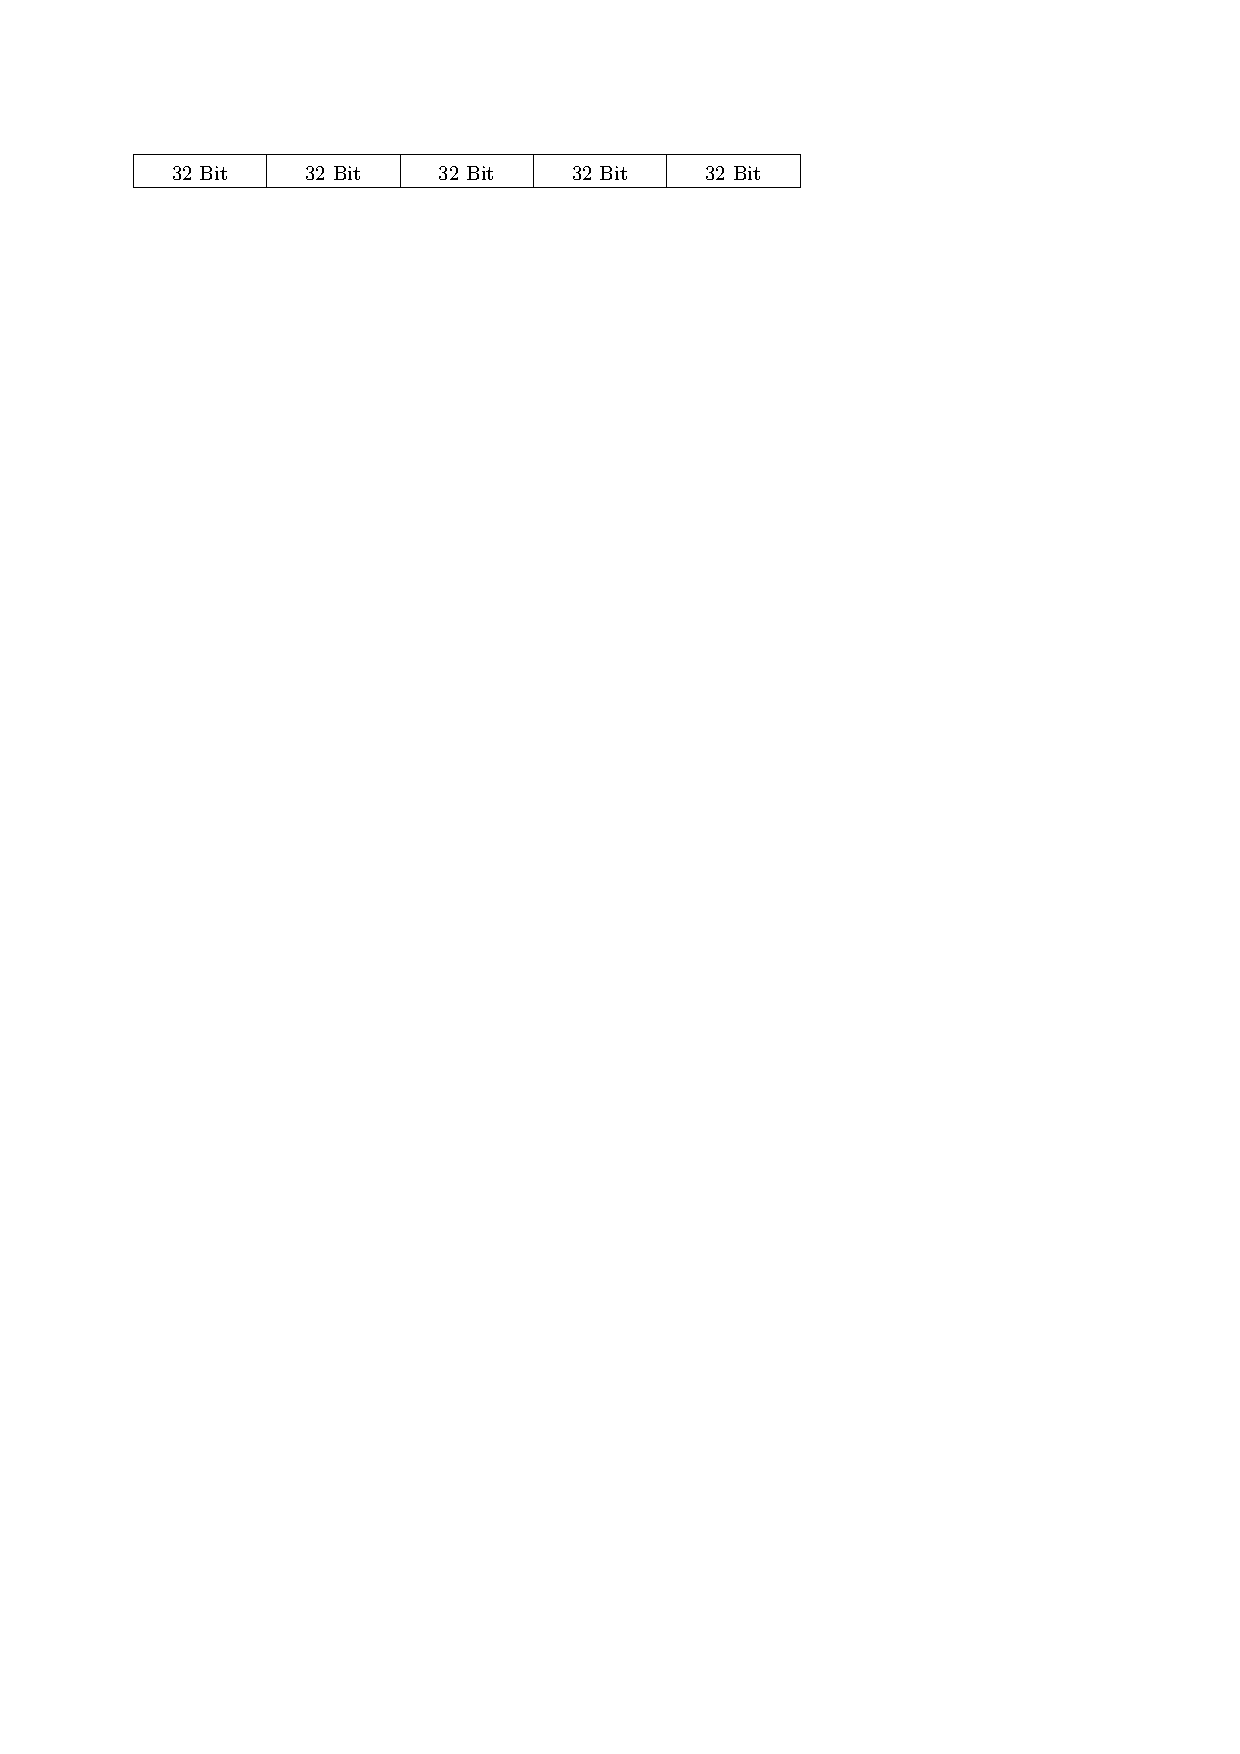
\includegraphics[width=\textwidth]{../GFX/VL4-32bit-blocks.pdf}
    \caption{32 Bit Blöcke, auf diesen Schulmethode anwenden}
    \end{center}
\end{figure}
$x=(x_{n-1}x_{n-2}...x_1x_0)_B = \sum\limits_{i=0}^{n-1}x_iB^i$\\
$y=(y_{n-1}y_{n-2}...y_1y_0)_B = \sum\limits_{i=0}^{n-1}y_iB^i$\\

%Einschub: Schulmethode\\
\begin{figure}[h!]
    \begin{center}
        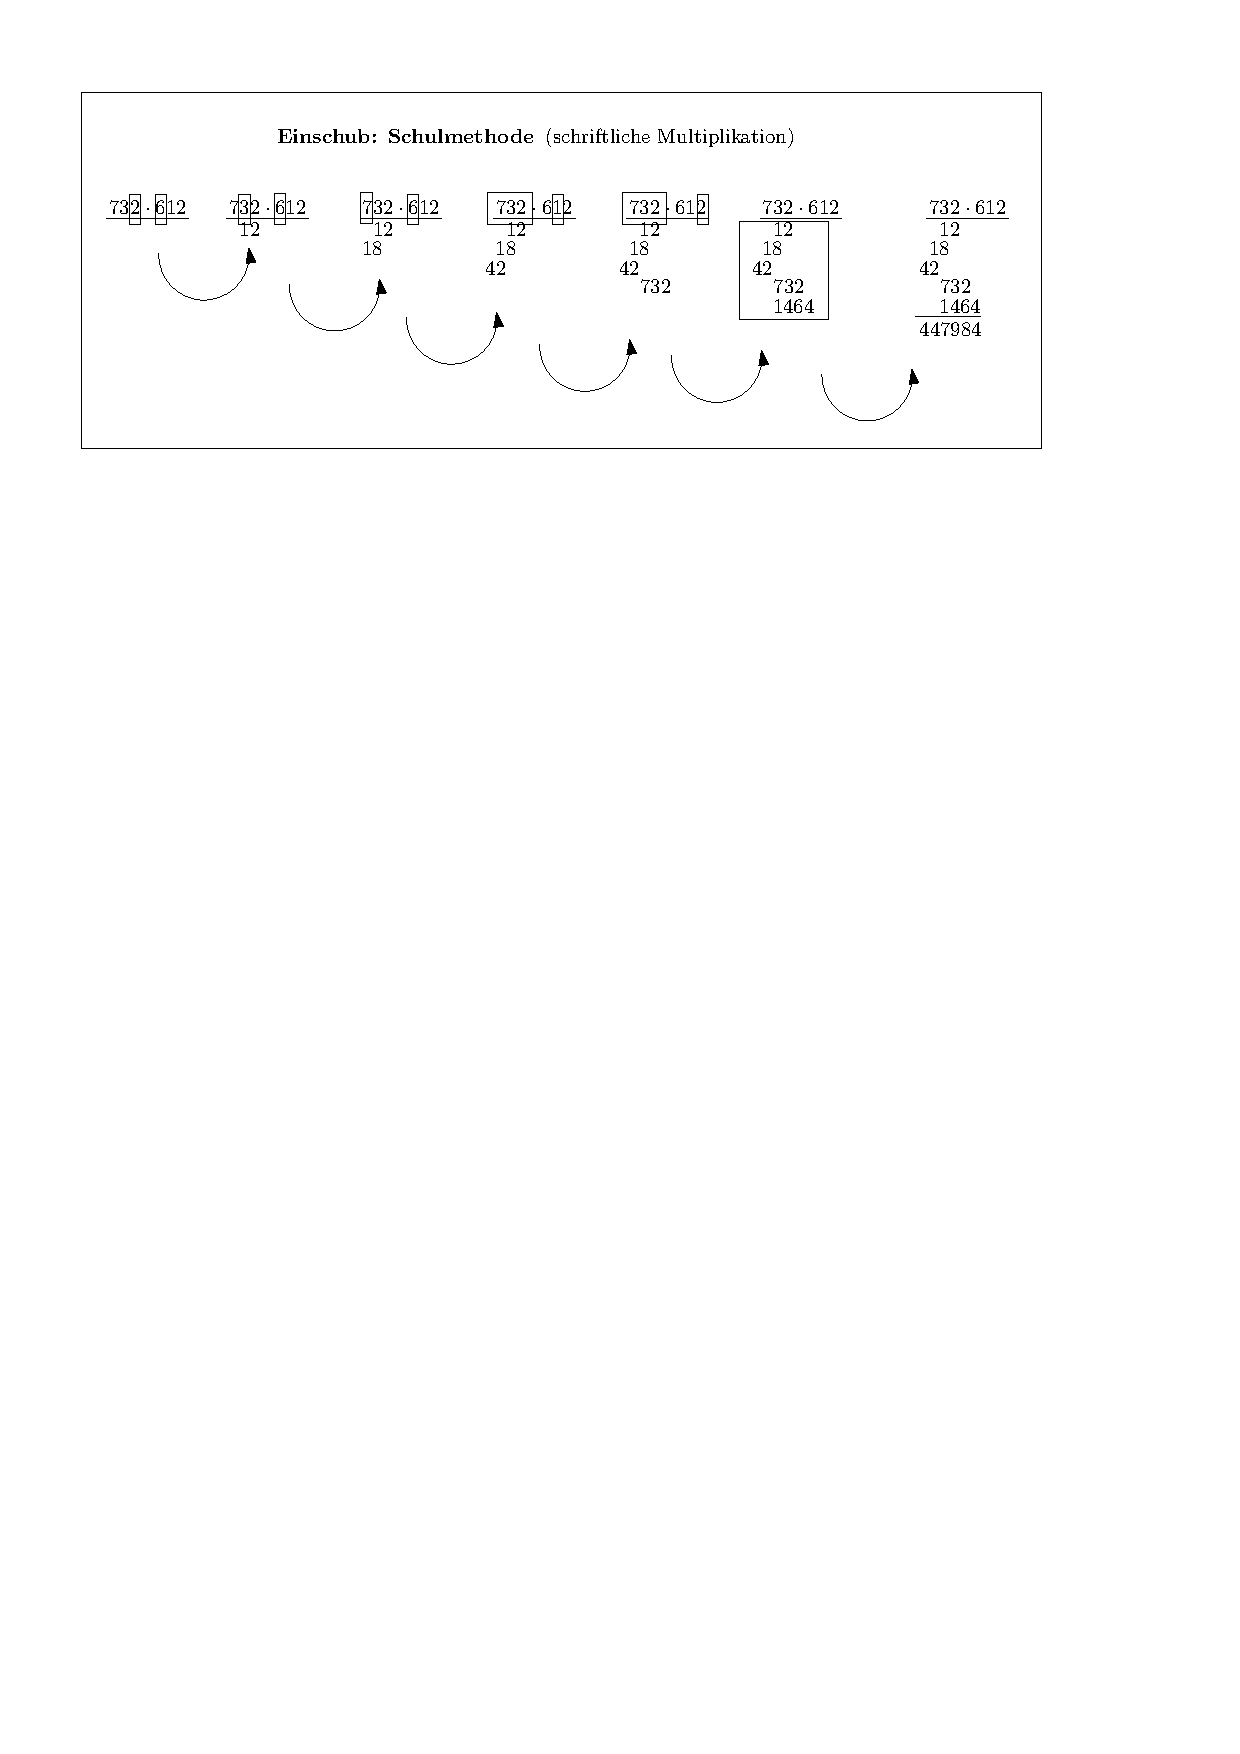
\includegraphics[width=\textwidth]{../GFX/vl4_fig_e1.pdf}
        \caption{Schulmethode (ohne Übertrag)}
        \label{fig:schulmethode}
    \end{center}
\end{figure}
%Ende Einschub

\textbf{Schulmethode:} Multipliziere jedes $x_i$ mit jedem $y_j$ und addiere alle Produkte an die geeignete Stelle (wie in Abbildung \ref{fig:schulmethode}).\\
\begin{align*}
    x\cdot y =\sum\limits_{i=0}^{n-1}\sum\limits_{j=0}^{n-1} x_iy_j\,B^{i+j} \text{  Laufzeit in }\mathcal{O}(n^2)
\end{align*}

\subsubsection*{Teile und herrsche (Basis $B=2$)}
\begin{figure}[h!]
    \begin{center}
        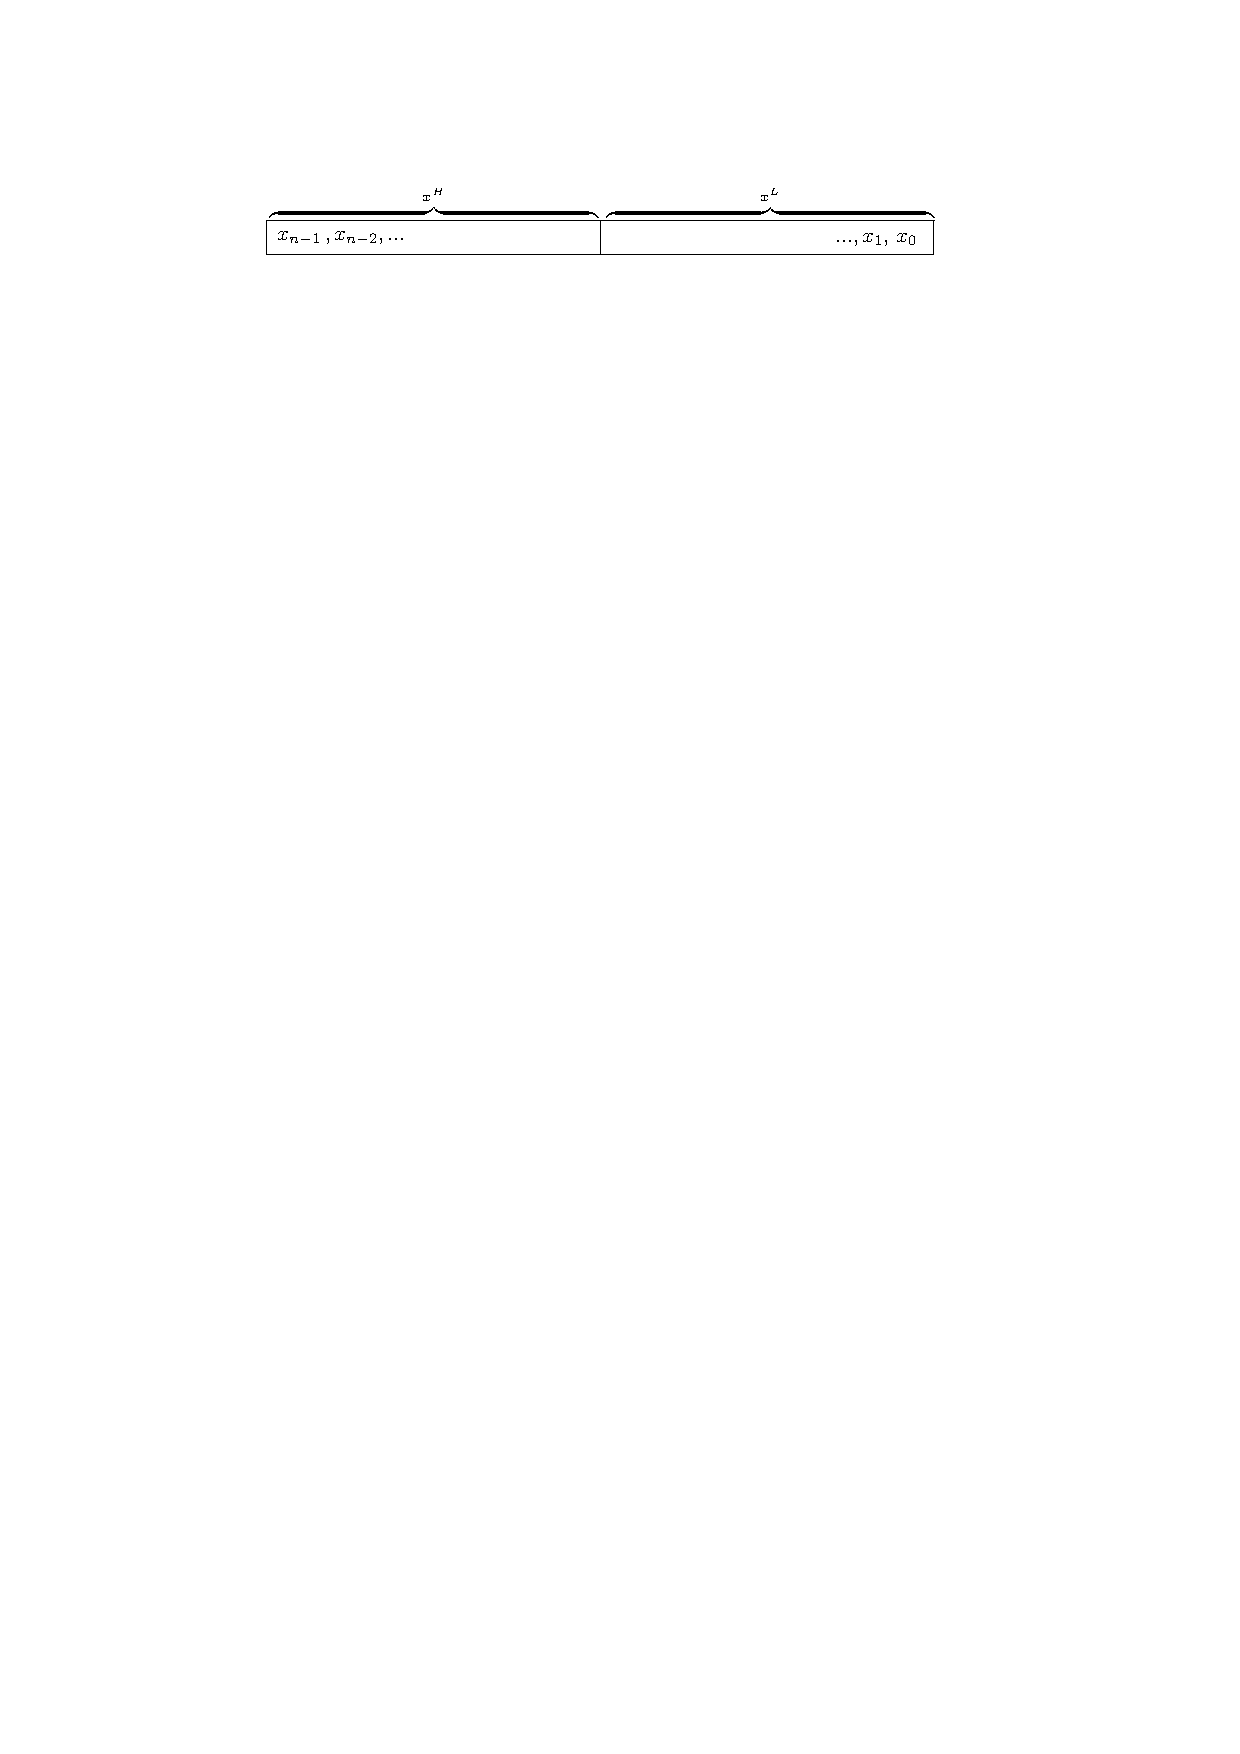
\includegraphics[width=\textwidth]{../GFX/VL4-hi-lo.pdf}
    \caption{Teile und herrsche}
    \label{fig:DaC}
    \end{center}
\end{figure}
Wie in Abbildung \ref{fig:DaC} zu sehen, sei $x$ eine $n$ Bit lange Zahl. Zur Vereinfachung nehmen wir an, dass $n$ gerade ist.\\
Wir teilen $x$ in zwei Teile, wobei ein Teil die höherwertigen Bits und der andere Teil die niedrigwertigen Bits enthält. Den Teil mit den höherwertigen Bits nennen wir $x^H$, den mit den niedrigerwertigen Bits nennen wir $x^L$.\\
Dann gilt $x= x^H\cdot 2^{\frac{n}{2}}+x^L$.\\
Außerdem sei $y$ eine entsprechend gewählte zweite Zahl für die gilt:\\
$y= y^H\cdot 2^{\frac{n}{2}}+y^L$\\


\begin{align*}
    x^H:&=(x_{n-1}x_{n-2}...x_{\frac{n}{2}})_2& \frac{n}{2}& \text{ höherwertige Bits }\\
    x^L:&=(x_{\frac{n}{2}-1}...x_0)_2 &\frac{n}{2}&\text{ niederwertige Bits}\\
    x &= x^H\cdot \underbrace{2^\frac{n}{2}}_{\text{Linksshift umi} 2^\frac{n}{2} \text{ Bits}}+x^L
\end{align*}


\begin{align*}
    xy&= (x^H\cdot 2^{\frac{n}{2}}+x^L)(y^H\cdot 2^{\frac{n}{2}}+y^L)\\
      &=x^Hy^H+(x^Hy^L+x^Ly^H)2^{\frac{n}{2}}+x^Ly^L\\
\end{align*}

\begin{align*}
    T(n)&=4T(\frac{n}{2})+\mathcal{O}(n)\\
\end{align*}
Diese Rekursion ist dargestellt in Abbildung \ref{fig:rekursion-schul}.\\
%Bild 4
\begin{figure}[h!]
    \begin{center}
        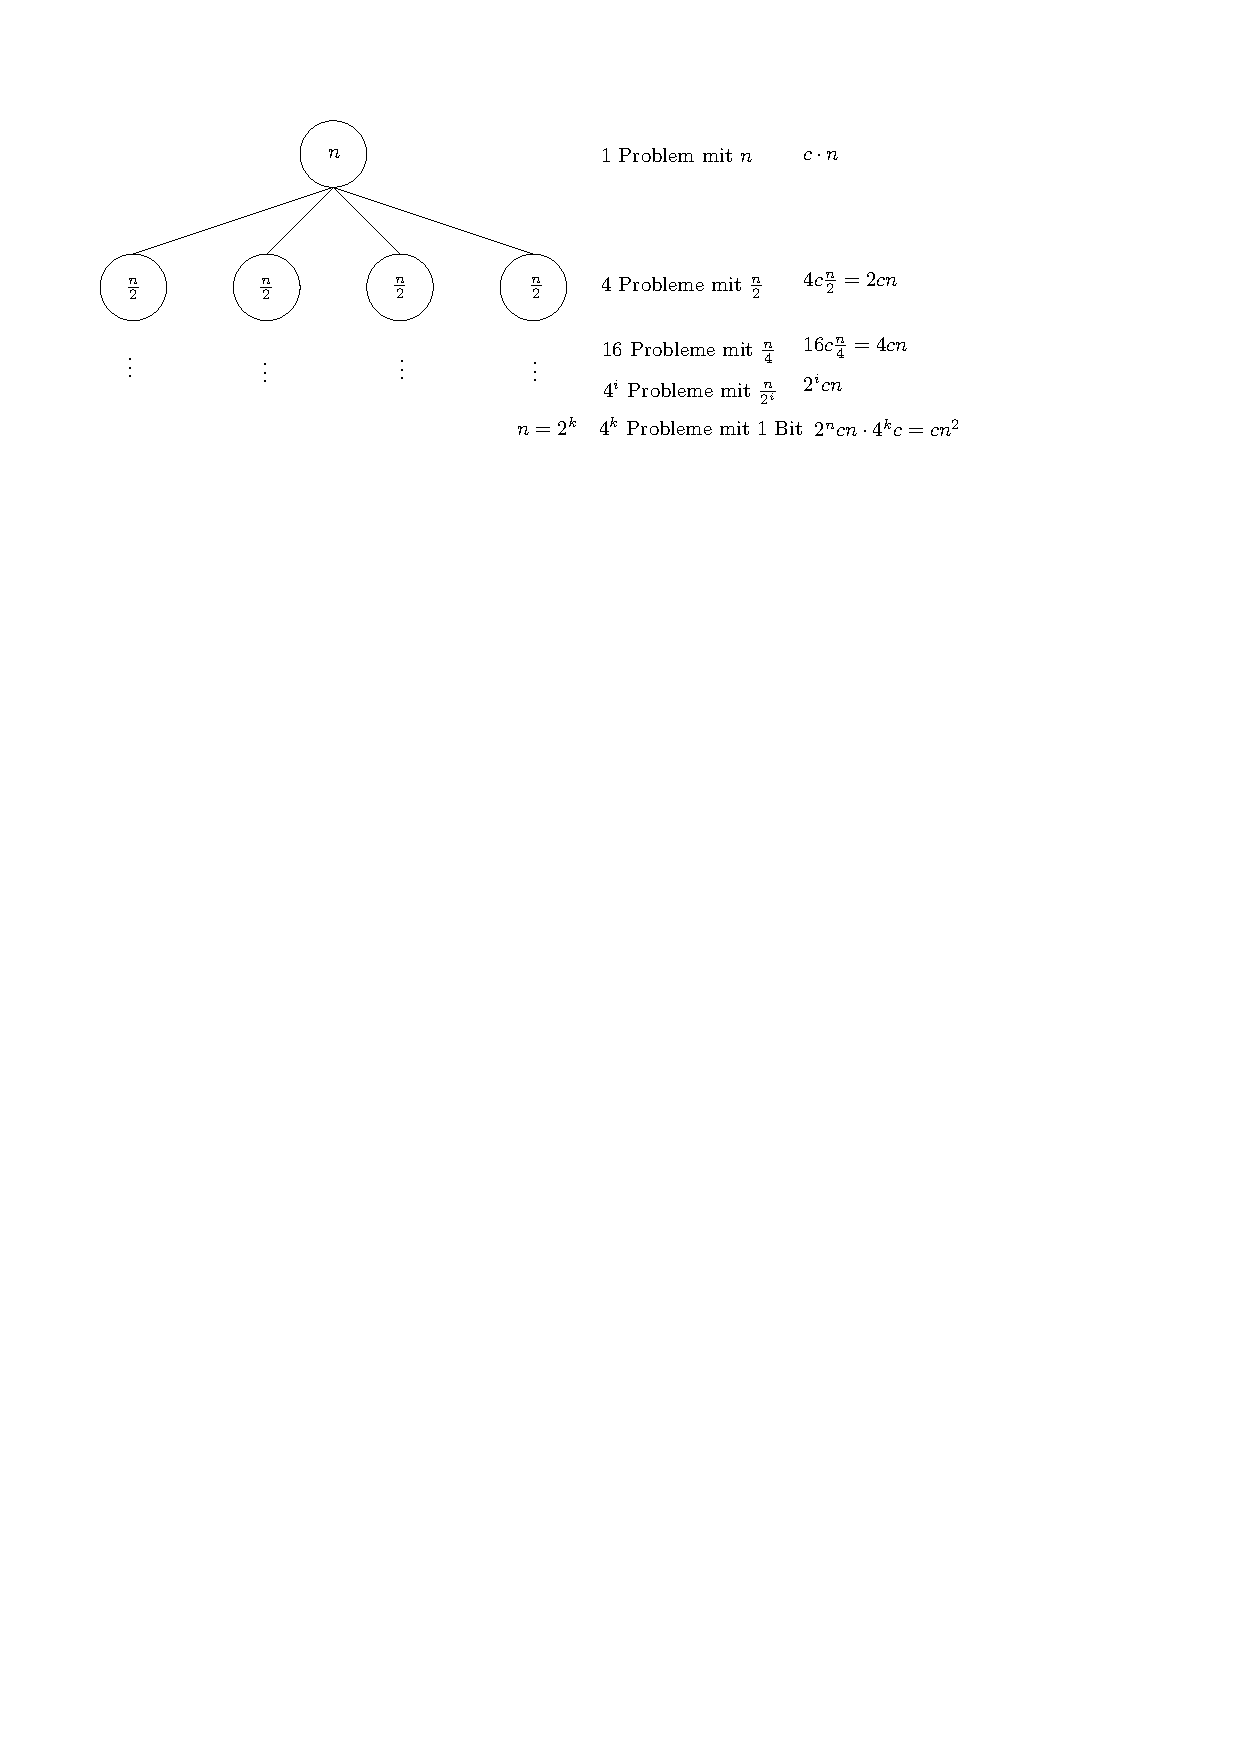
\includegraphics[width=\textwidth]{../GFX/vl4_fig_4.pdf}
        \caption{Rekursionsbaum - Schulmethode}
        \label{fig:rekursion-schul}
    \end{center}
\end{figure}

$\Rightarrow$ Laufzeit: $T(n)=\mathcal{O}(n^2)$\\
Somit ist bringt \glqq Teile und Herrsche\grqq in diesem Fall keine Verbesserung. Grund hierfür ist, dass wir vier Teilbäume haben.\\
Um eine Verbesserung zu erzielen, müssen wir die Anzahl der Teilbäume auf drei reduzieren.

\subsubsection*{Algorithmus von Karatsuba}
\textbf{Satz:} Es existiert ein Algoritmus, mit dem die Multiplikation zweier $n$-stelliger Zahlen in weniger als $\mathcal{O}(n^2)$ möglich ist.\\
Ein Algorithmus, der diesen Satz erfüllt ist der Algorithmus von Karatsuba.\\
Der Algorithmus von Karatsuba ist ein schneller Multiplikationsalgorithmus. Er reduziert für die Multiplikation zweier $n$-stelliger Zahlen die Anzahl der nötigen einstelligen Multiplikationen im Allgemeinen auf höchstens $3n^{\log_2 3}$. Für $n$ die ein Vielfaches von zwei sind sogar exakt auf $n^{\log_2 3}$. Damit ist er schneller als die klassische Schulmethode und erfüllt die Forderung aus dem vorangegangenen Abschnitt.\\
Der zugehörige Rekursionsbaum ist in Abbildung \ref{fig:karatsuba} dargestellt.\\
\begin{enumerate}
    \item $z_1 = (x^L+x^H)\cdot (y^L+y^H)= x^Ly^L+x^Hy^L+x^Ly^H+x^Hy^H$ (1 Multiplikation)
\item $z_2 = x^Ly^L$ (1 Multiplikation)
\item $z_3 = x^Hy^H$ (1 Multiplikation)
\item $z_4 = z_1- z_2 - z_3$
\item $xy= \underbrace{z_32^n}_{(*)}+z_4 2^{\frac{n}{2}}+z_2$
\end{enumerate}

(*) Diese Multiplikation kann durch shiften sehr effizient gemacht werden!

%Bild 5
\begin{figure}[h]
    \begin{center}
        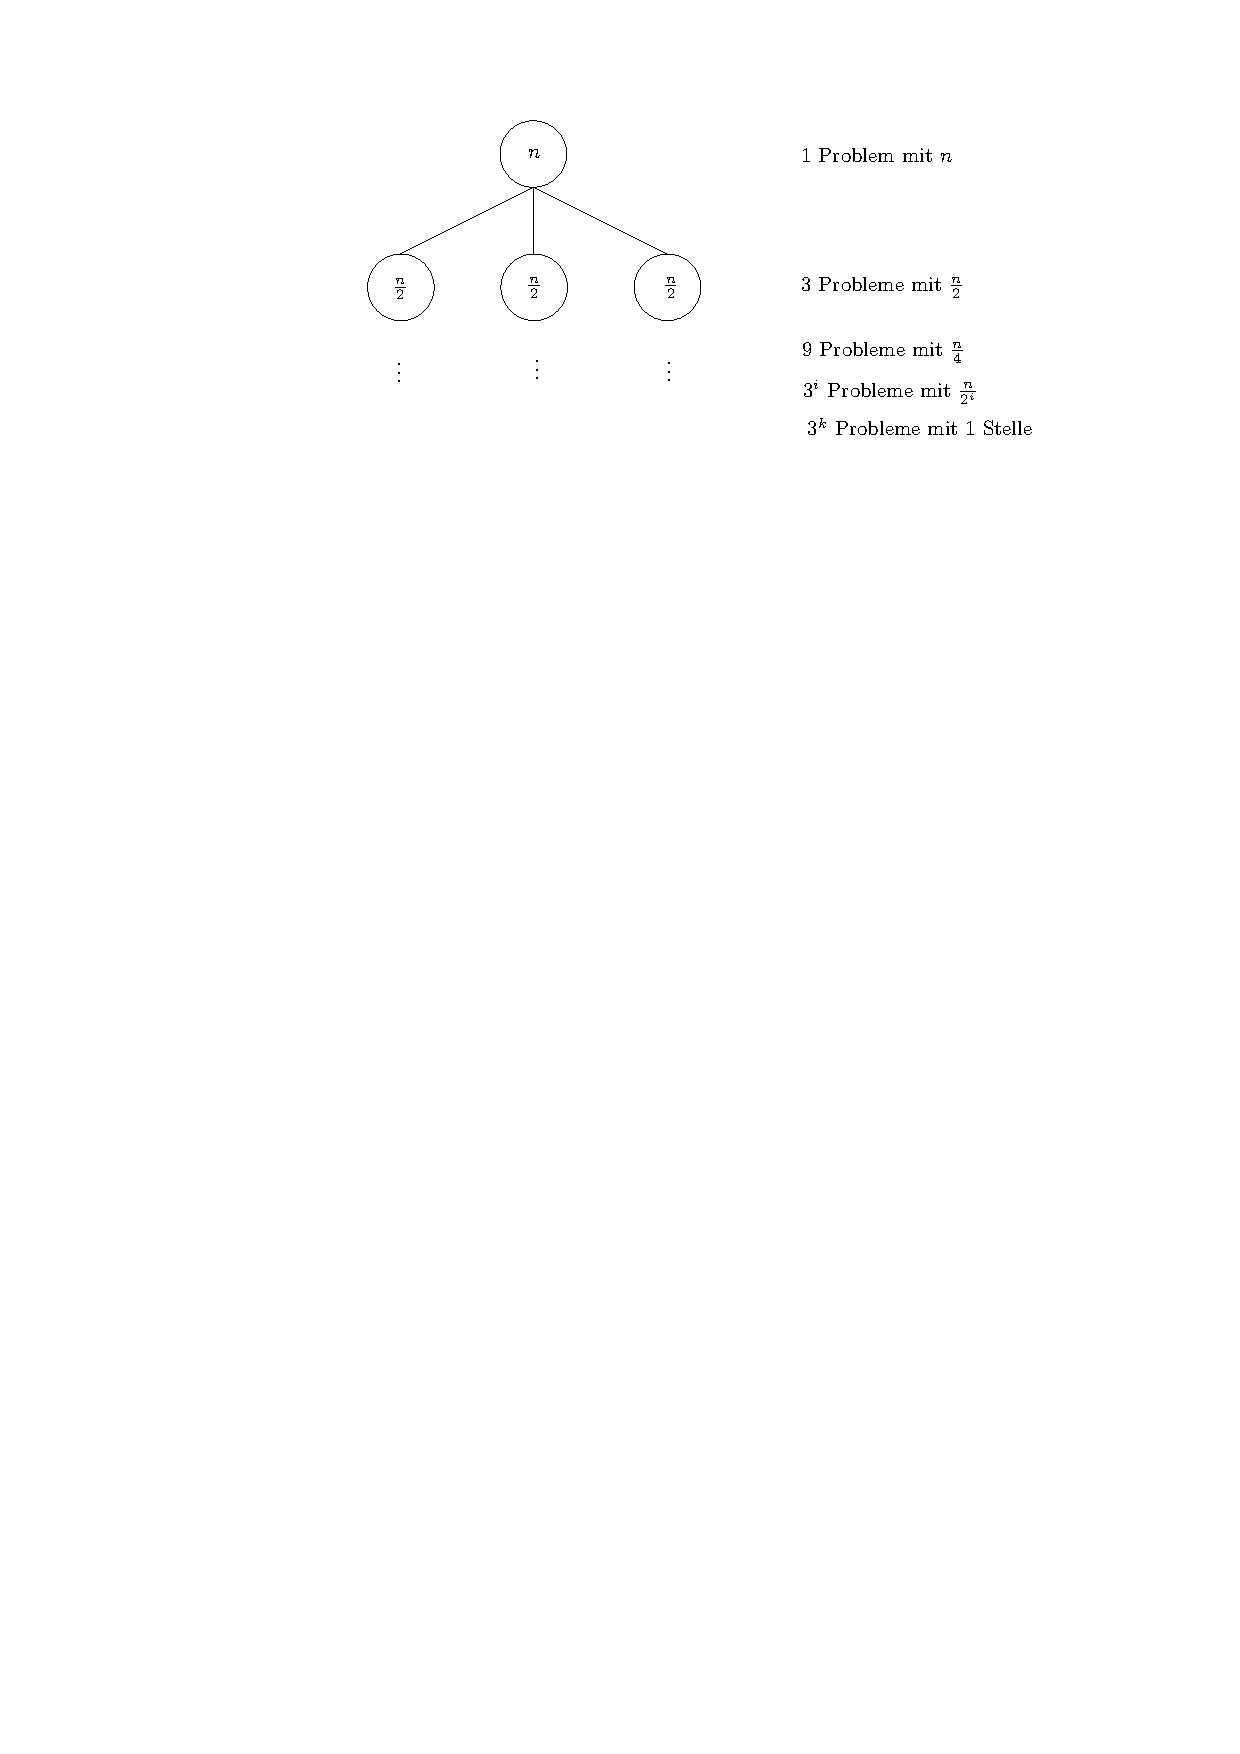
\includegraphics[width=12cm]{../GFX/vl4_fig_5.pdf}
        \caption{Rekursionsbaum - Algorithmus von Karatsuba}
        \label{fig:karatsuba}
    \end{center}
\end{figure}

Summiert man den Aufwand pro Ebene auf, erhält man für Ebene $i$ den Aufwand $(l\frac{3}{2})^i \cdot c \cdot n$. Summiert man die Ebenen auf, erhält man als Gesamtaufwand:\\
\begin{align*}
    &=\sum\limits_{i=0}^k \left(\frac{3}{2}\right)^i \cdot c \cdot n\\
    &=c\cdot n\cdot\sum\limits_{i=0}^k \left(\frac{3}{2}\right)^i\\
\end{align*}

Da diese Formel eine geometrische Reihe beschreibt, können wir eine endliche Partialsumme wie folgt berechnen:\\
\begin{align*}
    \sum\limits_{i=0}^k \left(\frac{3}{2}\right)^i&= \frac{\left(\frac{3}{2}\right)^{k+1}-1}{\frac{3}{2}-1}=\mathcal{O}\left(\left(\frac{3}{2}\right)^k\right)
\end{align*}
Für den Gesamtaufwand folgt hieraus:\\
\begin{align*}
    \Rightarrow c\cdot n\cdot\sum\limits_{i=0}^k \left(\frac{3}{2}\right)^i&=\mathcal{O}\left(c\cdot \not n \cdot \frac{3^k}{\not 2^k}\right)&\text{(Gilt, da } n=2^k\text{ )}\\
                                                                           &=\mathcal{O}\left(3^k\right)
\end{align*}

Da $3^k = 3^{\log_2n} = n^{\log_2 3}$ (Logarithmengesetzte), folgt:\\
\begin{align*}
    \mathcal{O}\left(n^\gamma\right)\text{, mit } \gamma = \log_2 3 \approx 1,7
\end{align*}
%\begin{align*}
%    T&=3^k\cdot c\\
%    T&=\mathcal(O)(3^k)\text{(geometrische Reihe mit Faktor }3\text{), } \leq \text{ größtes Glied }\frac{1}{1-\frac{1}{3}}=\frac{3}{2}\\
%    \log \frac{T}{c'} &= k \log 3 = \log n \frac{\log 3}{\log 2}\\
%    \log n &= k\log 2\\
%    k&= \frac{\log n}{\log 2}\\
%    \Rightarrow \frac{T}{c'} &= n^{\frac{\log 3}{\log 2}}=n^{\log_2 3} \approx n^{1,7}\\
%    T&=\mathcal{O}(n^\gamma), \gamma = \log_2 3\\
%\end{align*}
\textbf{Teile-und-herrsche-Rekursionen}\\
Die Strategie \glqq Teile-und-herrsche\grqq zerlegt ein Problem $T(n)$ in $a$ Teilprobleme der Größe $\frac{n}{b}$. Hinzu kommt der Aufwand für das Zerlegen in die Teilprobleme und Zusammenfügen derselbigen. Allgemein kann man also folgende Formel dafür angeben:\\
\begin{align*}
    T(n)&= a T(\frac{n}{b})+f(n)\\
%a &\text{ Teilprobleme der Größe } \frac{n}{b}\\
%f(n) &\text{ Aufwand für Zerlegen und Zusammenfügen}\\
\end{align*}

\newpage
\subsubsection*{MASTER-Theorem}
Das Master-Theorem, auch Hauptsatz der Laufzeitfunktionen, kann bei vielen rekursiven Funktionen, wie sie beispielsweise bei vielen Divide and Conquer Algorithmen auftreten, eine schnelle Einordnung in Laufzeitklassen ermöglichen.\\
%tab 1
\begin{center}
\begin{tabular}{|c|c|c|c|}
    \hline
    Anzahl Probleme& Größe & Aufwand&\\
    \hline
    $1$&$n$&$f(n)$&$n^4$\\
    $a$&$\frac{n}{b}$&$af(\frac{n}{b})$&$n^4\cdot \frac{a}{b^4}$\\
    $a^2$&$\frac{n}{b^2}$&$a^2f(\frac{n}{b^2})$&$n^4\cdot (\frac{a}{b^4})^2$\\
    $\vdots$&$\vdots$&$\vdots$&$\vdots$\\
    $a^k$&$\frac{n}{b^k}$&$a^kf(\frac{n}{b^k})$&$n^4\cdot (\frac{a}{b^4})^k$\\
    \hline
\end{tabular}
$$k=\log_b n$$
\end{center}
\begin{align*}
    \frac{n}{b^k}& \text{konstant, z.B. wenn }f(n) = n^4\\
\end{align*}

\textbf{3 Fälle:}\\
\begin{enumerate}
\item fallende geometrische Reihe: $(\frac{a}{b^4}<1)$: $T(n) = \mathcal{O}(f(n))$\\
\item wachsende geometritsche Reihe: $(\frac{a}{b^4}>1)$: $T(n) = \mathcal{O} (a^k) = \mathcal{O}(n^{\log_b a})$\\
\item konstant: $\frac{a}{b^4} = 1$: $T(n) = \mathcal{O}(n^{\log_b a} \log n)$\\
\end{enumerate}
